	\documentclass[12pt,a4paper]{book}
\usepackage[latin1]{inputenc}
%\usepackage{creativecommons}
\usepackage{xmpincl}
\usepackage{lipsum}
\usepackage{url}
\usepackage{amsmath}
\usepackage{amsfonts}
\usepackage{amssymb}
\usepackage{graphicx}
\usepackage{multicol}
\usepackage[normalem]{ulem} % needed by strike
\usepackage[urlcolor=blue,colorlinks=true]{hyperref}
\usepackage{makeidx}
\makeindex
\setcounter{tocdepth}{1}
\author{Paul Sutton}
\begin{document}

\begin{center}
{\Huge ToriOS Manual}
\end{center}



\begin{figure}
\centering
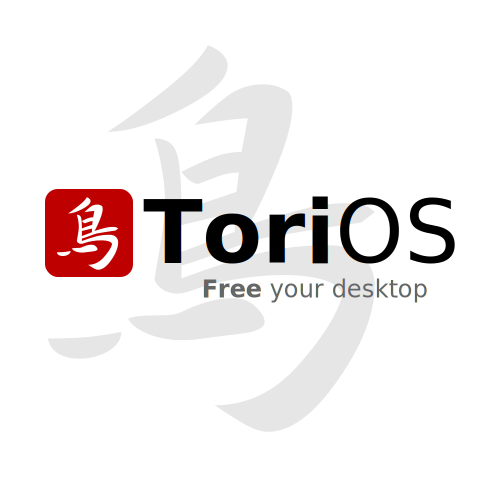
\includegraphics[width=0.7\linewidth]{./FinalLogo}

\end{figure}


\begin{center}
Minimal, Simple, Fast, Small and Gives you a freedom of choice :) \\
Manual by Paul Sutton
\end{center}

\tableofcontents
\index{Table of Contents}
\chapter{Introduction}
\index{Introduction}
The goal of this project is to produce a minimalist Linux distribution that gives end users more choice as to what software is installed on their system.\\

Ubuntu 12.04 is used as a base for this new system.
\subsection{About this Manual}
This manual refers to external websites to help explain concepts further, to avoid the need to reproduce what is already out there.  The ToriOS team take no responsibility for external content.  The links are correct and suitable at the time of writing,  Broken links are out of the Authors control between revisions.  It is your responsibility to ensure suitability of information, you should read fully and seek other sources of information and ask for help if unsure.  
This manual has been prepared using \LaTeX.

\chapter{What is GNU / Linux}

Linux refers to the kernel of the operating system.  GNU refers to the tools used with Linux and the licensing model these are released under,  GNU stands for GNUs Not Unix,  so these are versions of the tools you would find on the UNIX operating system but released under a free license in this case the GPL (General Public license).
\index{GNU}
\index{Linux}
\index{GNU / Linux}
\index{GPL}
\subsection{About ToriOS}
\index{About ToriOS}
ToriOS is a system aimed at replacing Windows XP, which has reached end-of-life as of April 2014. ToriOS is a fast and minimal system based on Ubuntu 12.04. 

\subsection{Non PAE Support}
\index{PAE}
\index{Non PAE}

PAE - Physical Address Extension.\\
To quote Wikipedia - In computing, Physical Address Extension (PAE) is a feature to allow 32-bit IA-32 central processing units (CPUs) to access a physical address space (including random access memory and memory mapped devices) larger than 4 gigabytes.  \\




ToriOS will support PAE Hardware\\
https://blueprints.launchpad.net/torios/+spec/non-pae-support

\newpage 
\subsection{Technical overview}
\index{Technical overview}
About Tori OS - Tori Operating System Overview:

\begin{itemize}
\item{Low memory and resource requirements}
\item{Low disk space}
\item{Low package overheads (you get to build your own system from a very minimal install base)}
\item{Built with Ubuntu 12.04LTS as a base , and completely compatible with many thousands of free and paid apps.}
\item{ A modern OS with up-to-date security built-in, as well as compatible with older processors and video graphics cards}
\item{Free and open source}
\item{A secure replacement for older unsupported versions of Microsoft Windows Operating System} 
\end{itemize}


\chapter{The ToriOS Team}
\index{The Team}
\begin{center}\begin{tabular}{|l|l|l|l|}
\hline \textbf{Job Title} & \textbf{Name} & \textbf{IRC Nick} & \textbf{E-mail} \\
\hline Project lead & Ali Linx & amjjawad & amjjawad@torios.org \\
\hline Website admin & William Cornelius &  & william@torios.org \\
\hline Documentation - manual & Paul Sutton & zleap	& zleap@torios.org \\
\hline Documentation - wiki & Geoffrey De Belie & smile & smile4ever@torios.org \\
%\hline Developer lead / driver & Alexander Kluth & DerAlex & alexander@torios.org \\
\hline Quality Assurance Testing & Jack & fjack & $|$ \\
\hline Marketing $|$	David B Yentzen & $|$ dbyentzen@torios.org \\
\hline Artwork & Rafael & rafaellaguna & $|$ \\
\hline Developer / testing & Israel & israeldahl & israel@torios.org \\
\hline \end{tabular}\end{center}


\chapter{Installation - Getting ToriOS}
\index{Installation}
There are several steps to an installation. \\
\begin{enumerate}
\item decide on the installation media CD-R or Flash disk
\item Prepare install media - in the case of a flash disk make sure this is blank
\item Prepare target media and decide where to install Torios to
\item Download the iso file
\item Create your install media
\item initial boot
\item either install from menu or run live session and install from there


\end{enumerate}

\subsection{Downloading the ISO}
\index{Downloading - CLI}
\subitem{Command Line}

See chapter \ref{Testing} for how to download and test the iso. 

\subitem{Browser}
\index{Downloading - Browser}

\text{You can also download using a web browser}

\subsection{Verifying the download}
There is an excellent guide at\\ \textbf{https://help.ubuntu.com/community/HowToMD5SUM} \\
that explains how to check your downloaded iso file for errors.  Apart from the file name being different so for ToriOS you may have ToriOS-1.0.0.iso the steps are pretty much the same.  
Please see getting involved section as this covers some of the above during the testing phase,  that information will appear here once the test phase is over. 
\chapter{Creating install media}

\subsection{CD-R}
\index{CD-R/RW/DVD-R/RW}

When you have an ISO file or disk image you need to BURN image to cd.  When using which ever cd mastering program you have.  If you copy to CD you will have a cd with an ISO file on it.  You won't be able to boot from that media.

\subsection{Flash Disks - Unetbootin}
\index{Flash Disks}
\index{Unetbootin}
You can use unetbootin to create a bootable flash disk image,   

See the URL ref section for links to the unetbootin website \ref{URL REF}

You can follow the steps below \\

Creating a boot usb flash disk

(With thanks to Nio Wiklund for some helpful comments with regard to the title of this document)

A good tool for this is Unetbootin,  you can install this on most popular Linux distributions,

e.g sudo apt-get install unetbootin

you need your root password.

You can then load the software up, you will need your root password

Unetbootin as well as mkusb works in most linux distros, but I think
it is also very important, that Unetbootin works in Windows (and I
think also in MacOS). Please write very clearly, at or near page 16,
that Unetbootin can be installed in Windows and used to create a
ToriOS boot USB pendrive/stick/flash/thumb drive (whatever name you
prefer, or all of them).

http://unetbootin.sourceforge.net/

\newpage




\begin{center}
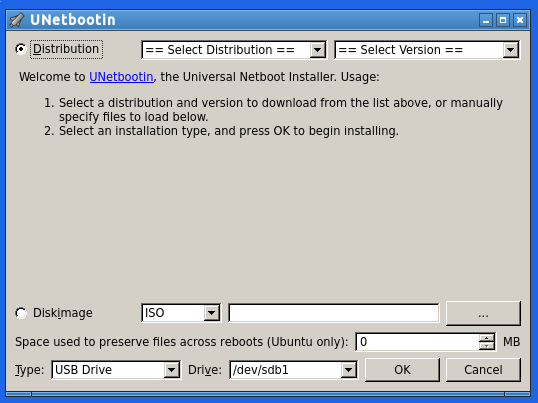
\includegraphics[width=0.7\linewidth]{unetbootin} 
\end{center}


If you have downloaded an iso image  you don?t need to worry about the top section

Click disk image,  ISO can be left as in,  then click the box with ? in and select the iso file

select type, usb drive or hard disk,  most people are going to want to create a usb boot flash disk.

drive should be the device reference for this disk

make sure you are 100 percent sure,  and if you are not sure ASK on forums , IRC or elsewhere first.

I find it helpful to unmount and unplug my external hdd first,  it gives less options but also reduces the chances I will write to it,  The disks tool below is useful for finding out what device you are writing to.

If you have already downloaded and md5 checked your iso file then you don?t need to worry about the top part,

Click disk image radio button

the drop down menu to the right of this is a betweet ISO and floppy

you can then click on file search button (the one with ? )
\begin{center}
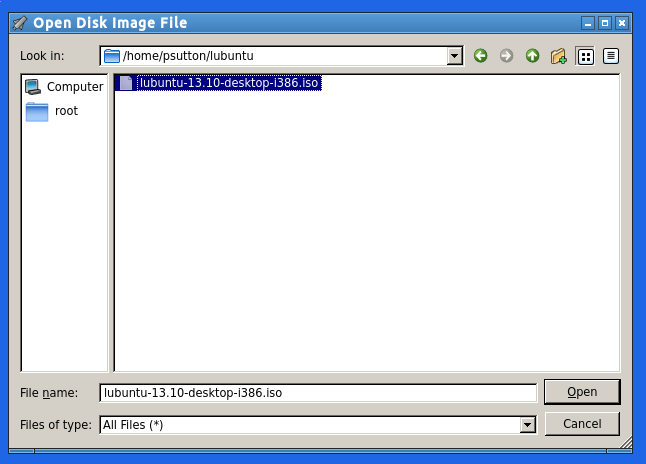
\includegraphics[width=0.7\linewidth]{unetbootin2} 

\end{center}



Select if you want to have a persistent space for files.


\begin{center}
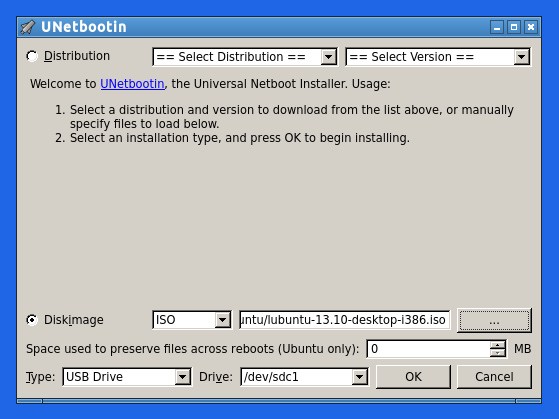
\includegraphics[width=0.7\linewidth]{unetbootin3}
\end{center}

Type? you can choose between usb and hard disk \textbf{BE VERY CAREFUL} //

then select the device, if you select hard disk then the device reference chances to / indicating root of the file system. //

\textbf{REMEMBER} that you can wipe your whole file system if you get the options wrong,  if you have an external hard disk and a usb disk plugged in I find it helpful to unmount and unplug the external hard disk,  gives less target options and is less likely to get wiped by mistake. //

 
\begin{center}
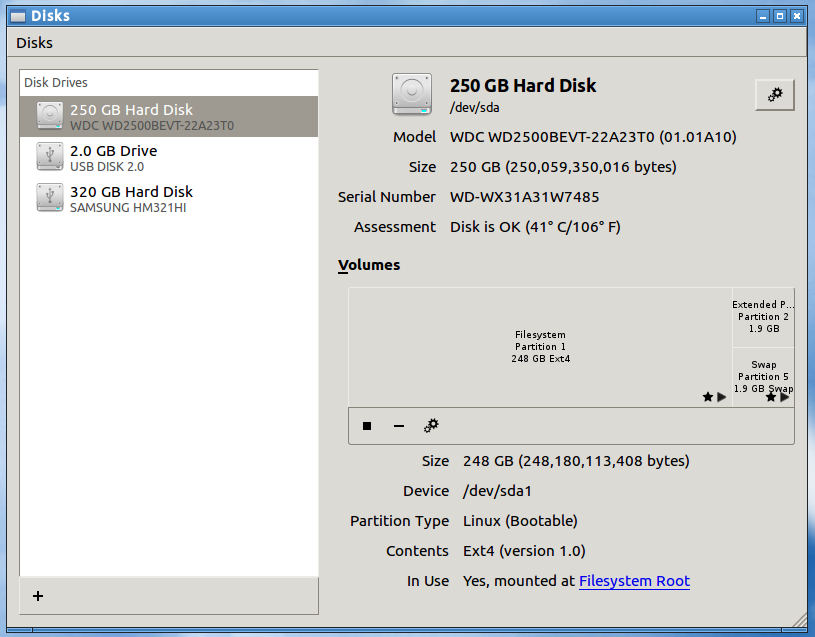
\includegraphics[width=0.7\linewidth]{unetbootin4}
\end{center}
You need to check if the target device should be mounted first or not


\paragraph{Hopefully this how to is useful,  please be careful as I am not responsible for data loss,  I try and write guides to be generic not explicit guides.  I will leave this to the documentation team}

\paragraph{You can use fdisk and df to determine device references. Read the man pages for more info if you get stuck as for help and say you have looked at man pages,  this blog post etc and are still stuck,  this shows you have tried to research the issue.}

The ubuntu manual should have this information in it too.

man unetbootin

man fdisk

man ls

man df

If you need to format the flash disk, using disks, this is a case of

Unmount the flash disk

Select format

MAKE SURE YOU HAVE THE RIGHT DEVICE SELECTED.

Once this is all done and you are happy with the destination click OK

Progress bar showing how many files have been copied and a percentage


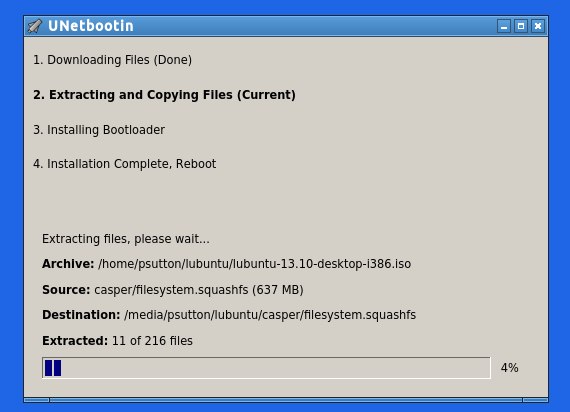
\includegraphics[width=0.7\linewidth]{unetbootin5} \\

All done you can now reboot, select usb disk from the boot device menu (see your Manual on how to access this) and tryout /  install the new OS

\text{unetbootin also works from Windows / Mac}

\subsection{Flash Disks - mkUsb}
\index{MkUSB}
\text{mkUSB - Make USB}

See the URL ref section for links to the information on mkusb \ref{URL REF}

mkusb is split now into one GUI program 'mkusb' and two console or text
applications, mkusb-nox and mkusb-bas. The GUI version works in ToriOS
(as well as in Ubuntu, Fedora, Debian, openSUSE. Arch to mention a few
distros).

mkusb-nox 'can do what mkusb can' but without eye-candy. mkusb-bas is
basic and can be used in simple distros, where certain tools are not
available (I have tested and tweaked it to work in Wary Puppy and Tiny
Core).

http://phillw.net/isos/linux-tools/mkusb/mkUSB-quick-start-manual.pdf

http://phillw.net/isos/linux-tools/mkusb/mkUSB-quick-start-manual-nox.pdf

http://phillw.net/isos/linux-tools/mkusb/mkUSB-quick-start-manual-bas.pdf

\newpage 

\chapter{BOOTING INSTALL MEDIA}

\text{Depending on how your computer is set up,  you need to tell the computer to boot of which ever boot media you created either a) cdrom b) dvd c) usb.} //

\subsection{UEFI Boot}
If you have very new hardware then you may have the new UEFI boot system,  this means you can't just boot the install media and there are a few extra steps.  These are outlined here.

\newpage

\section{Installation}

\subsection{Installing Torios One Button Installer}
\index{OBI}
https://help.ubuntu.com/community/OBI\\
For more help with the One button installer please refer to the OBI-quickstart-manual.pdf
\\
\textbf{Note ; This is based on the RC-2 test version.}
\linebreak \\
I set up virtual box with the default settings (256mb RAM)and added a 16gb virtual hard disk sda. \\
\\
First step in the process is to boot the iso image,  this automatically boots in to the new ToriOS desktop

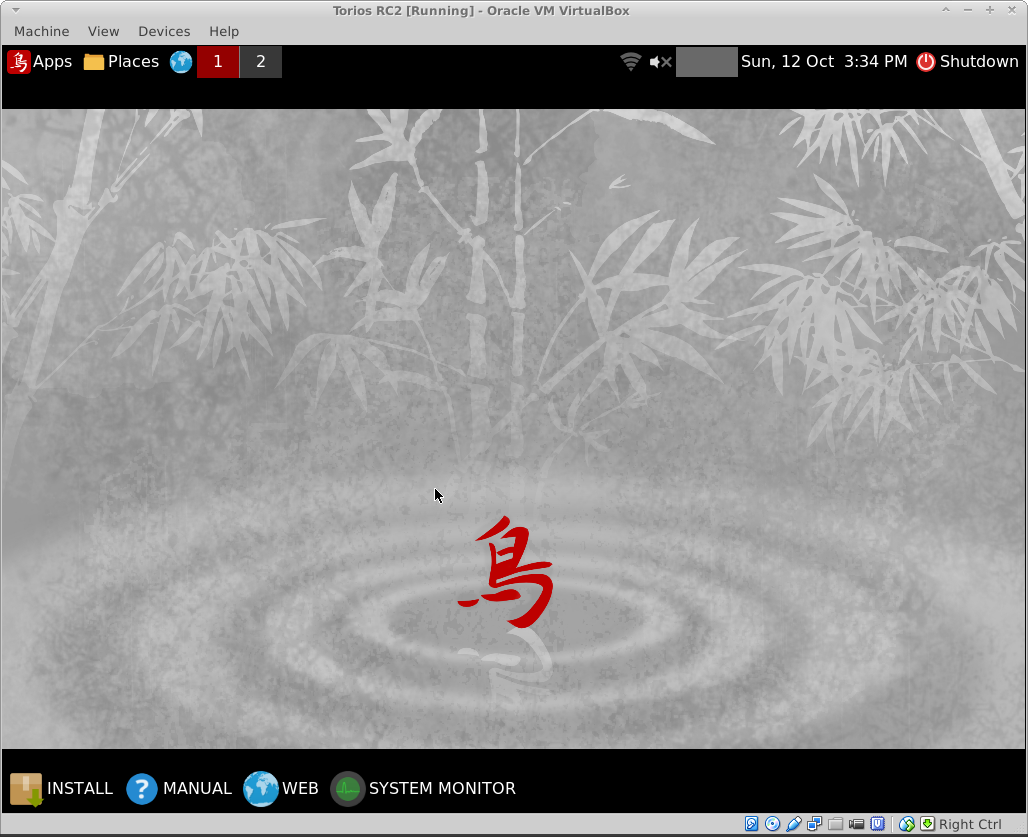
\includegraphics[width=0.7\linewidth]{toriosRC2} 
\\

Note the install button at the http://phillw.net/isos/linux-tools/mkusb/mkUSB-quick-start-manual.pdfbottom of the screen,  click this to start the install process. \\
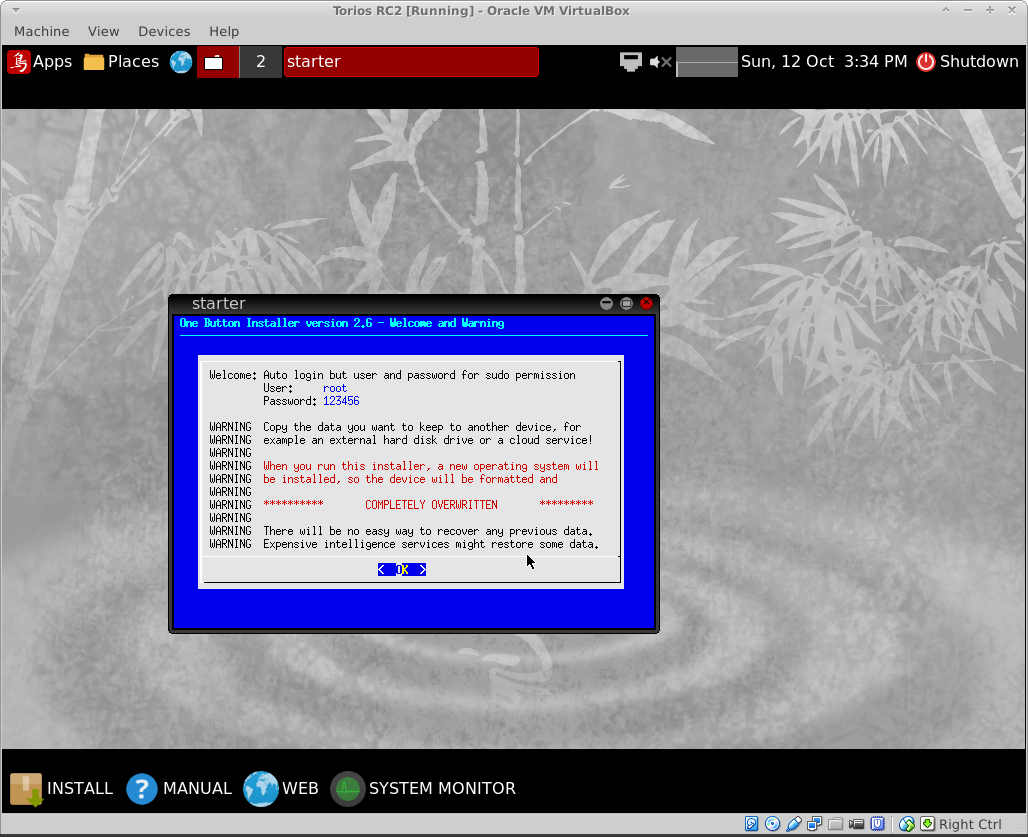
\includegraphics[width=0.7\linewidth]{torios-rc2-install1}

The initial screen is show here,  i accepted all the defaults except right at the very end for the confirm, where I had to manually select (yes) \\

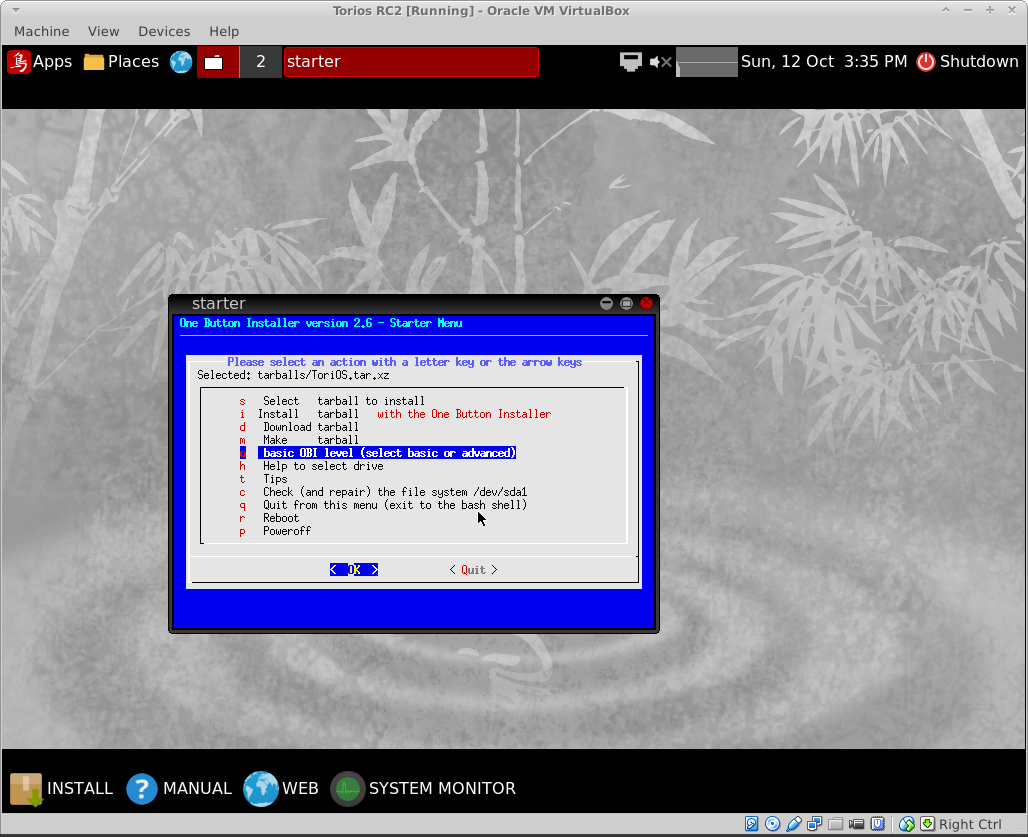
\includegraphics[width=0.7\linewidth]{torios-rc2-install2}

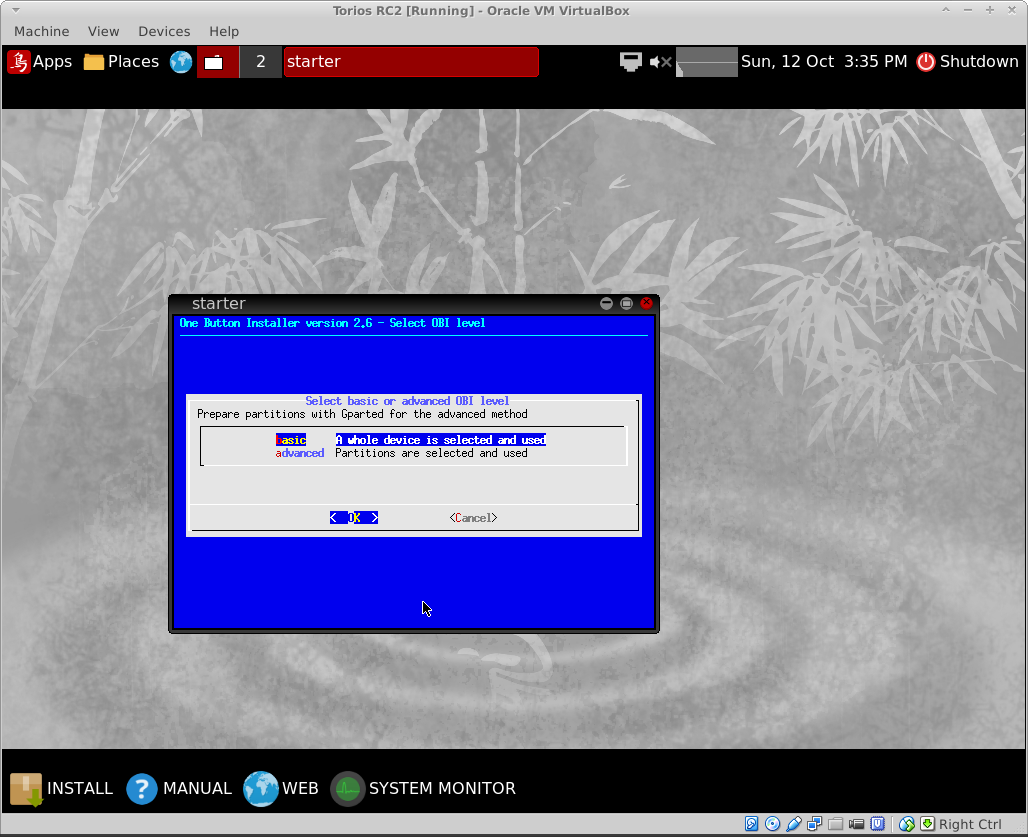
\includegraphics[width=0.7\linewidth]{torios-rc2-install3}

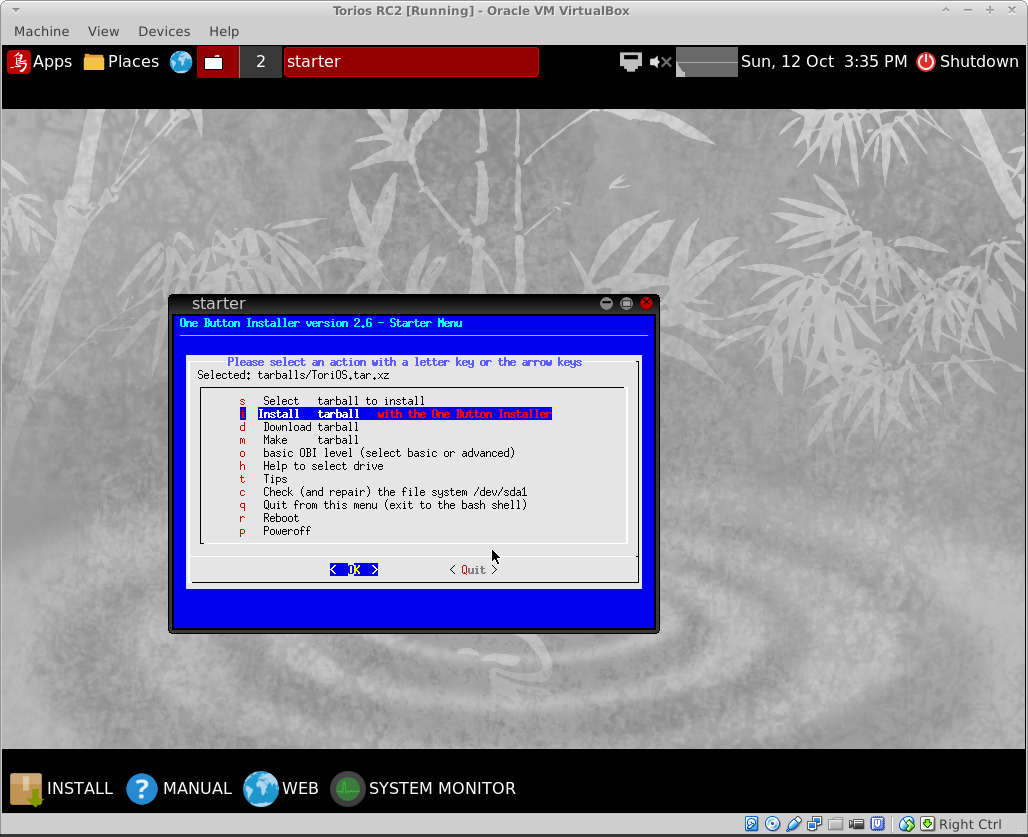
\includegraphics[width=0.7\linewidth]{torios-rc2-install4}

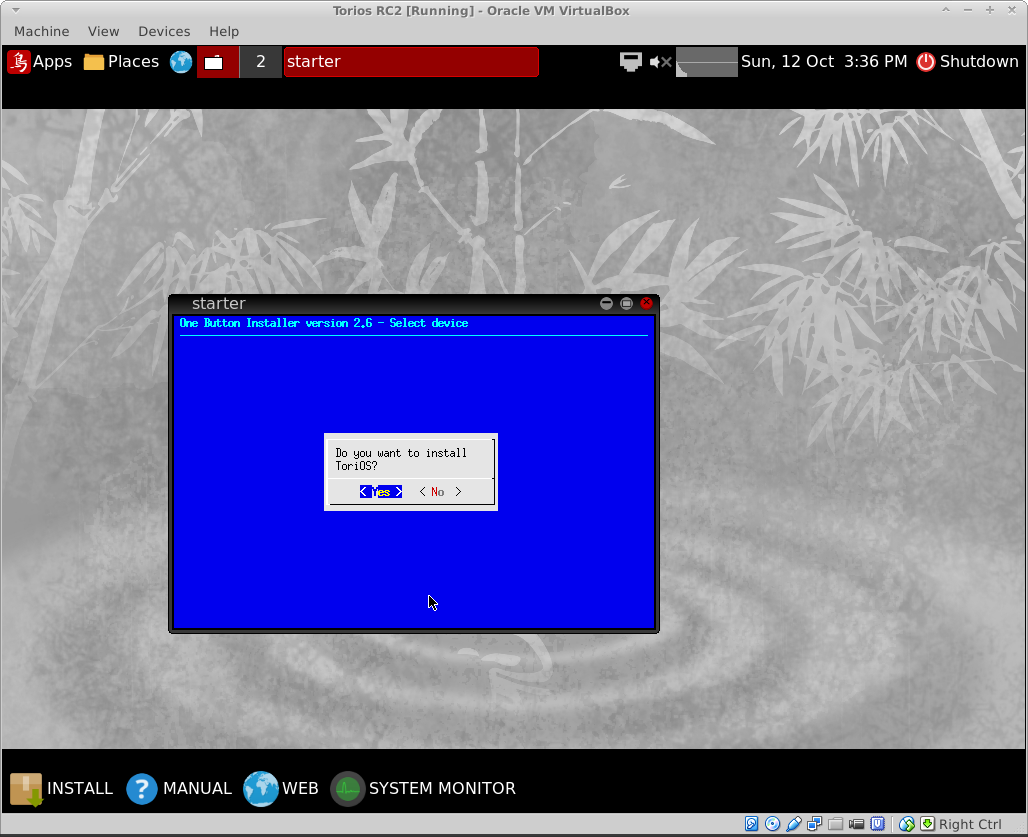
\includegraphics[width=0.7\linewidth]{torios-rc2-install5}

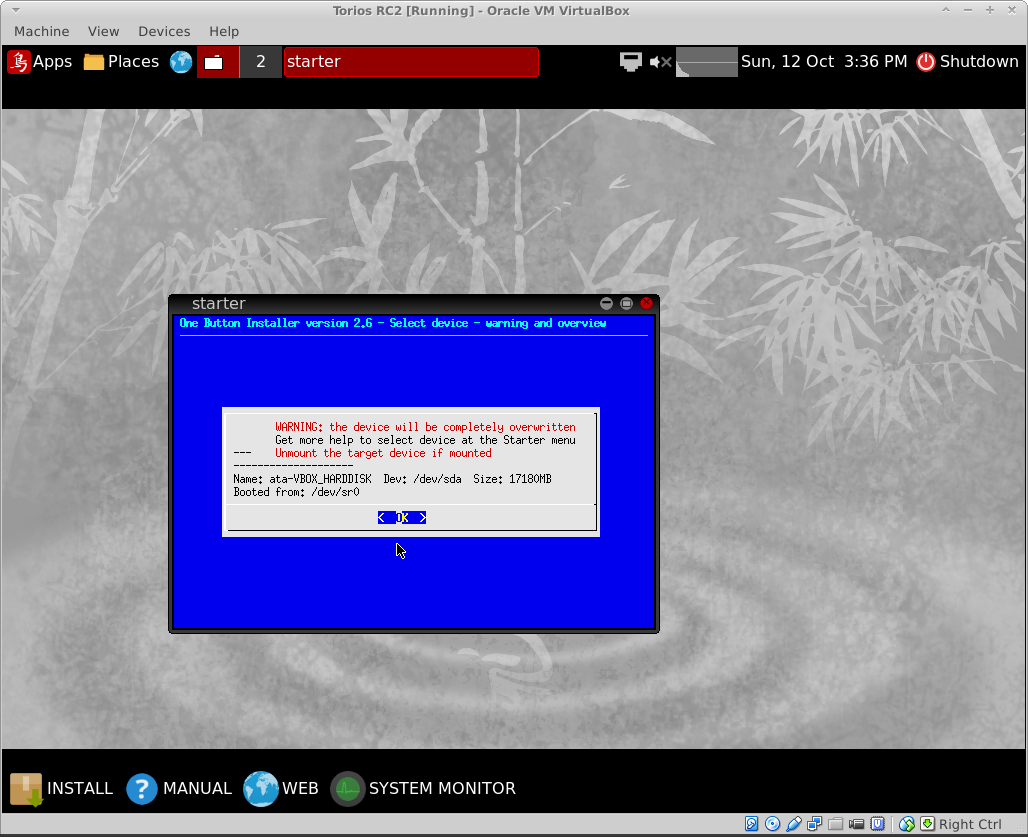
\includegraphics[width=0.7\linewidth]{torios-rc2-install6}


the next screen has a FINAL RED warning. \\ 

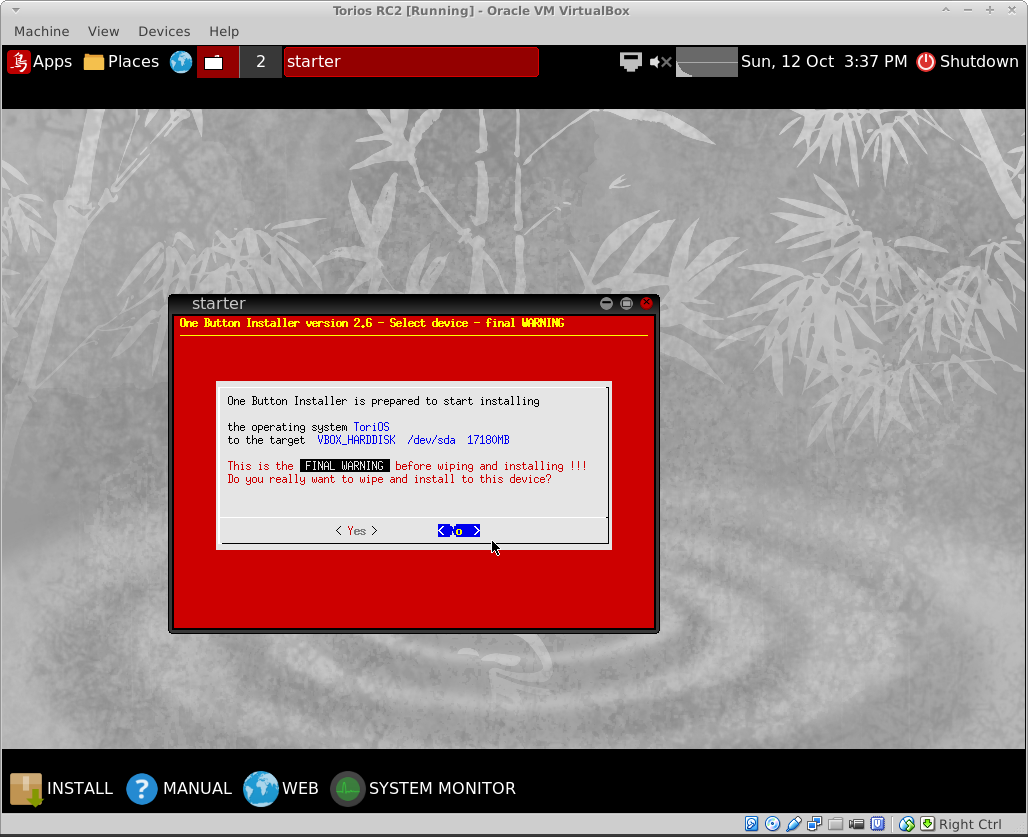
\includegraphics[width=0.7\linewidth]{torios-rc2-install8-final-warning}
%\includegraphics{torios-rc2-install8-final warning}

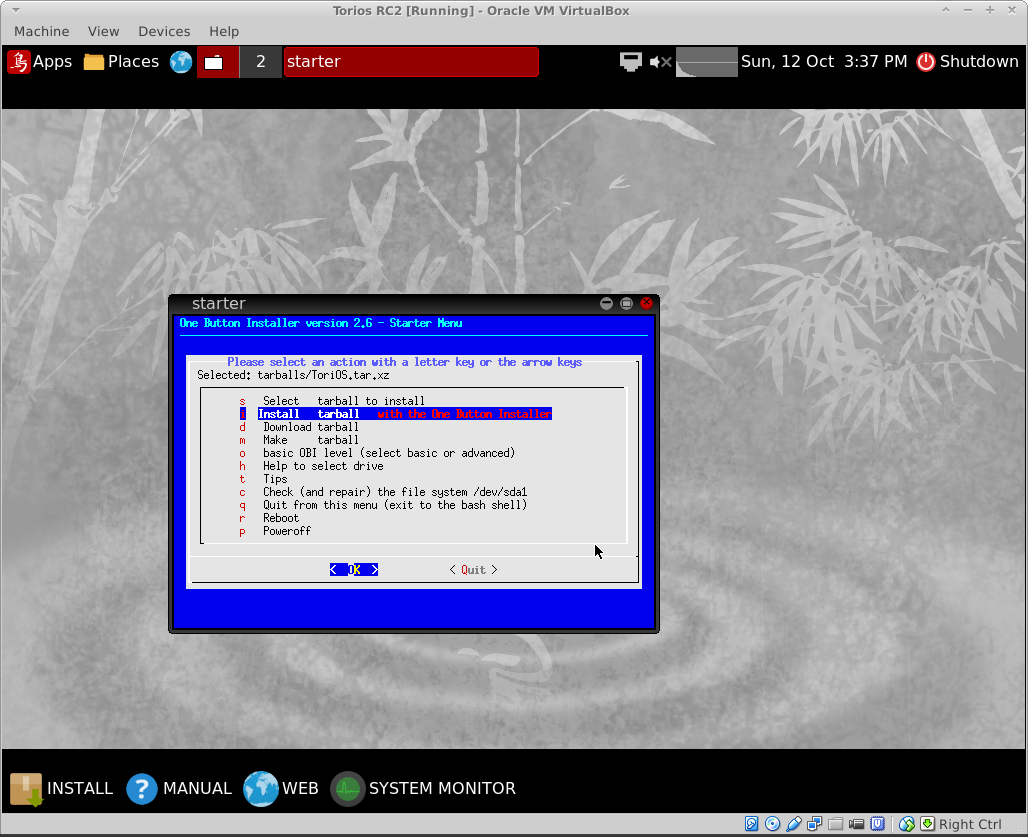
\includegraphics[width=0.7\linewidth]{torios-rc2-install9}


%\includegraphics[width=0.7\linewidth]{torios-rc2-login-screen}


\includegraphics[width=0.7\linewidth]{screen-shots/torios-rc2-login-screen}
%end install section

 
\newpage

\chapter{Login}

\includegraphics[width=0.8\linewidth]{screen-shots/torios-rc2-login-screen} \\

After booting you will be presented with a graphical login screen :

\chapter{Logout}

\text{Logging out of ToriOS}\\
\text{Click the shutdown menu in the top right corner}\\
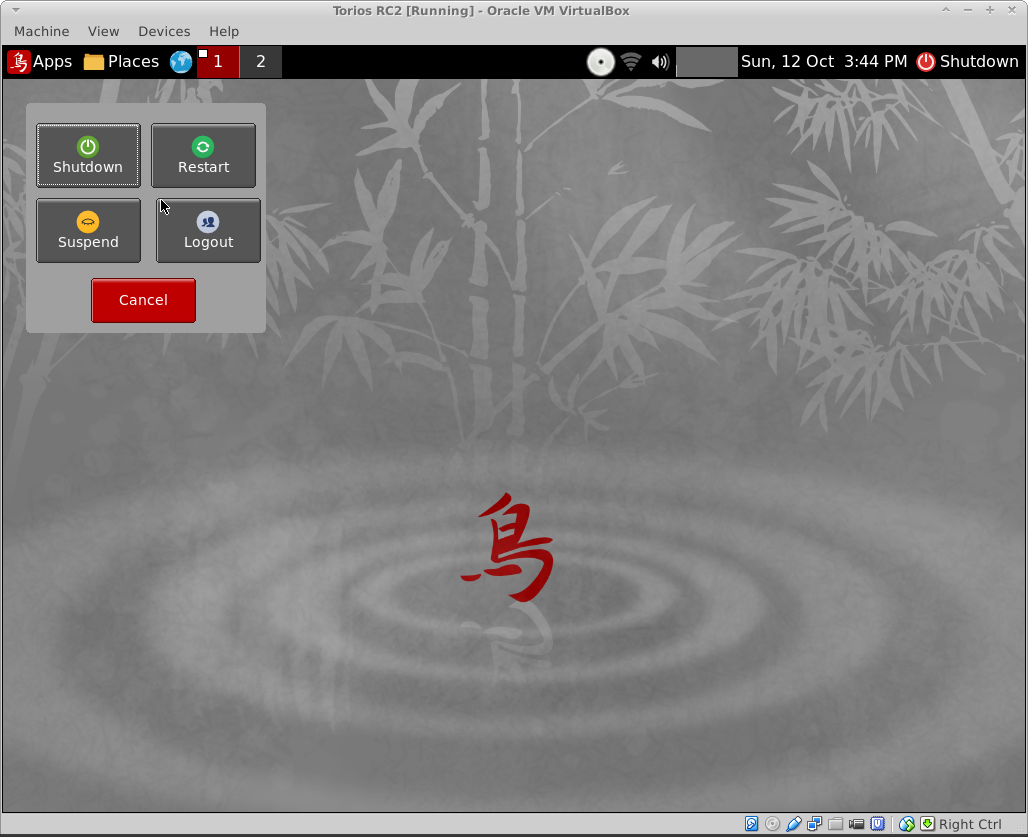
\includegraphics[width=0.8\linewidth]{screen-shots/torios-rc2-shutdown-menu} 
Here you are presented with 4 options:\\
\begin{itemize}
\item{Shutdown}
\item{Suspend}
\item{Logout}
\item{Restart}

\end{itemize}

\newpage 

 
\chapter{Desktop}

\text{Once you are logged in you should see the desktop}\\


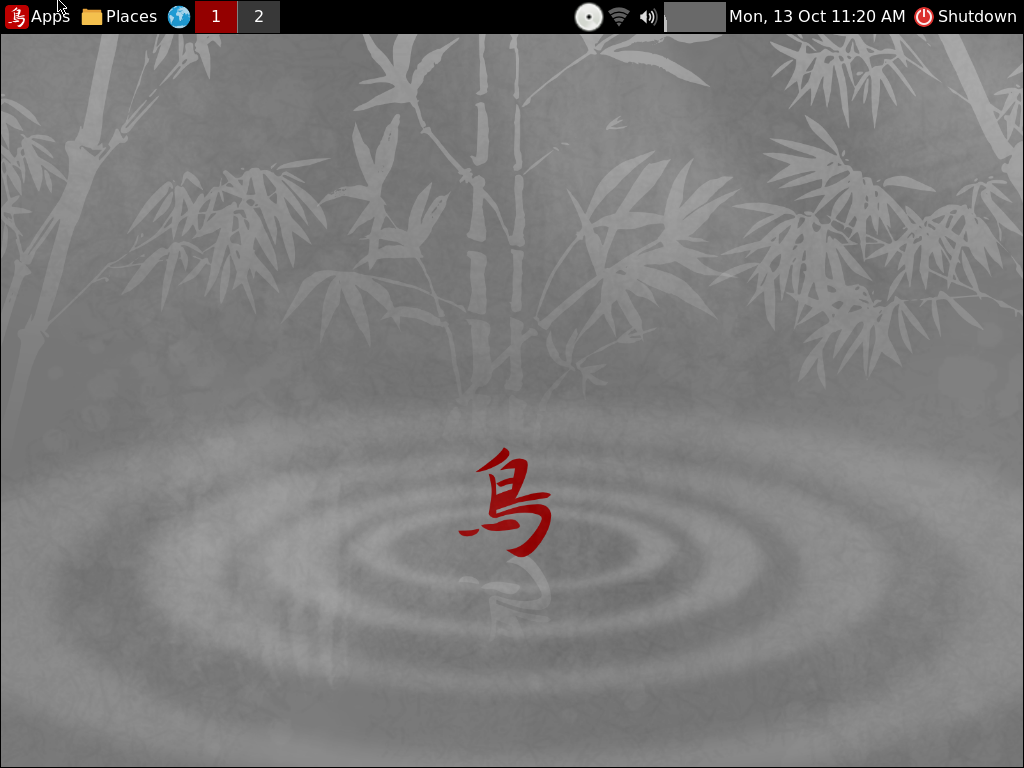
\includegraphics[width=0.8\linewidth]{screen-shots/Torios_Alpha2-desktop}

\chapter{Shortcuts}
\index{Shortcuts}
\begin{center}\begin{tabular}{|l|l|}
\hline \textbf{KEY} & \textbf{FUNCTION} \\
\hline F12 & Fullscreen \\
\hline Mute Key & Mute \\
\hline RaiseVolume Key & Raise Volume \\
\hline LowerVolume Key & Lower Volume \\
\hline WWW Key & Webbrowser \\
\hline PrintScr & Screen Shot - whole screen \\
\hline Ctrl+Alt+p &	Screen Shot \\
\hline Ctrl+Alt+t &	 Open Terminal \\
\hline Ctrl+Alt+Delete & Open System Monitor \\
\hline Alt+Tab & Switch to the next stacked window \\
\hline Ctrl+Alt+Tab & Cycle to the next stacked window \\
\hline Alt+F4 &	Close the window \\
\hline Alt+\# & Move to Desktop \# \\
\hline Alt+F1 &	Main Menu \\
\hline Alt+F2 & Unmaximize a window \\
\hline Alt+F10 & Maximize a window \\
\hline Ctrl+Alt+Right & Move Right 1 Desktop \\
\hline Ctrl+Alt+Left & Move Left 1 Desktop \\
\hline Ctrl+Alt+Up & Move Up 1 Desktop \\
\hline Ctrl+Alt+Down & Move Down 1 Desktop \\
\hline Ctrl+Alt+q &	close \\
\hline \end{tabular}
\end{center}

\textbf{This is work in progress}


\chapter{Applications}
As previously stated ToriOS is desgined to be very very minimal however it does come with a few applications. 

\subsection{seamonkey (Web browser)}
\index{Seamonkey}
\subsection{seamonkey (Private Browsing)}
\subsection{Wicd Network Manager}
\subsection{WPA-gui}
\subsection{ART Menu}
\newpage
\subsection{Evince}
\index{Evince}


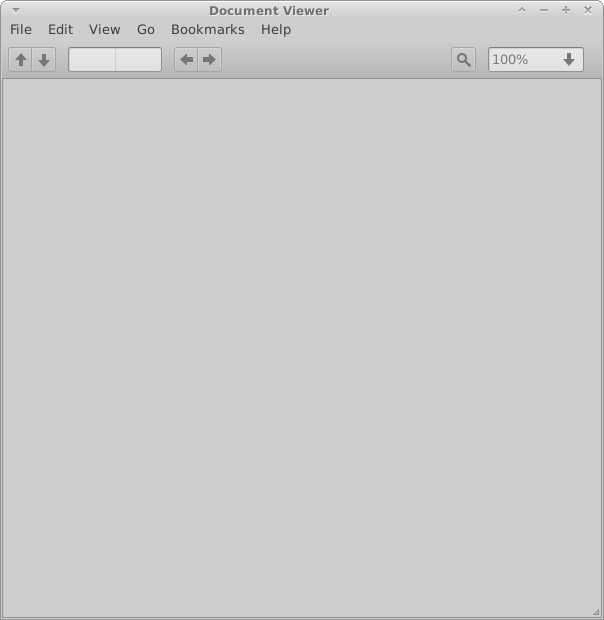
\includegraphics[width=0.8\linewidth]{screen-shots/evince}
\\
Document (PDF) Viewer
\\
\begin{center}\begin{tabular}{|l|l|}
\hline \textbf{ITEM} & \textbf{DESCRIPTION} \\
\hline Application name & Evince \\
\hline Application Description & PDF Viewer \\
\hline Menu Name & Document Viewer \\
\hline Installed Version & 3.4 \\
\hline Screen Shot version & 3.10.3 \\
\hline Screen Shot Source & xubuntu 14.04 \\
\hline Website & \htmladdnormallink{https://wiki.gnome.org/Apps/Evince}{https://wiki.gnome.org/Apps/Evince} \\
\hline \end{tabular}\end{center}



\newpage 
\subsection{Development}
\subsection{(Python 2.7)}

\subsection{Settings}
\subsection{GParted}
\index{GParted}
\subsection{JWM Settings Manager}
\subsection{Power Manager}

\subsection{System}
\subsection{UXTerm}
\subsection{XTerm}
\subsection{Htop}



\subsection{JWM Settings}
\index{JWM Settings Manager}
ToriOS will use the JWM (Joe's Window Manager) window environment:\\

The following is quoted from the projects website

\begin{quote}
JWM is a light-weight window manager for the X11 Window System. JWM is written in C and uses only Xlib at a minimum. Because of its small footprint, JWM makes a good window manager for older computers and less powerful systems, such as the Raspberry Pi, though it is perfectly capable of running on modern systems. JWM is included in small Linux distributions such as Puppy Linux and Damn Small Linux, and it is available as a separate package in many other distributions. 
\end{quote}
http://www.joewing.net/projects/jwm/
Torios jwm development lead Israel israel@torios.org
ToriOS Site Page : http://torios.org/jwm.html
\newpage

{\large \textbf{JWM Settings manager}} \\ \\


\begin{center}
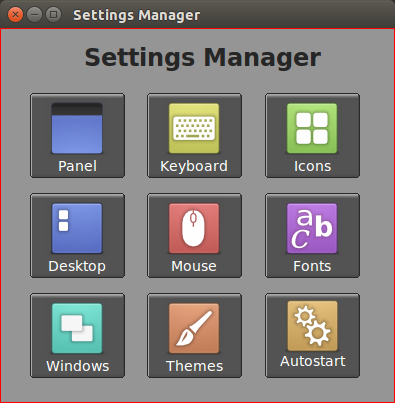
\includegraphics[width=0.7\linewidth]{jwmsettingsmanager}
\end{center}

\begin{center}
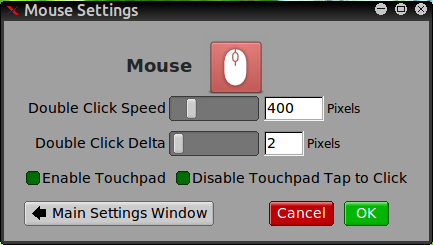
\includegraphics[width=0.7\linewidth]{mouse-settings}
\end{center}

\begin{center}
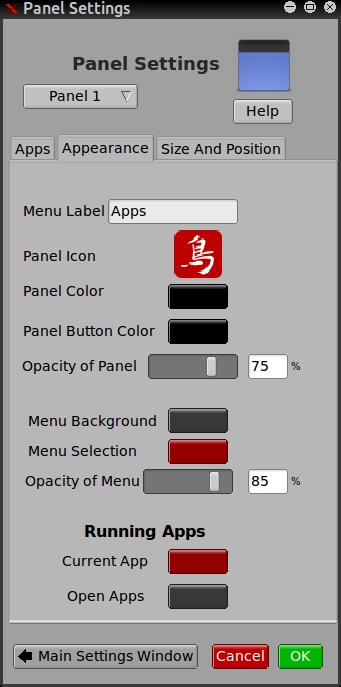
\includegraphics[width=0.7\linewidth]{panel-settings}
\end{center}


\begin{center}
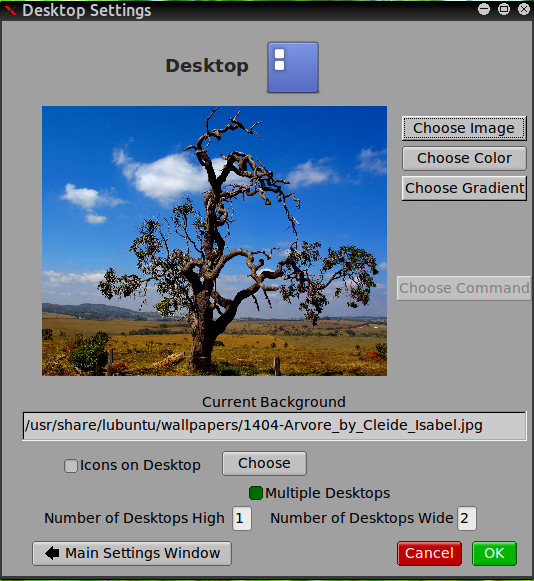
\includegraphics[width=0.7\linewidth]{desktop-settings}
\end{center}

\begin{center}
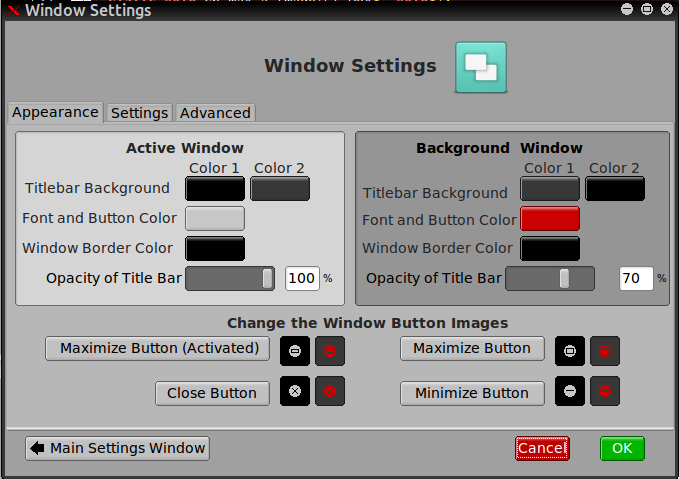
\includegraphics[width=0.7\linewidth]{window-settings}
\end{center}
%{Panel}

%{Keyboard}
%{Icons}

{Windows}
{Themes}
{Autostart}


\newpage

\subsection{}

\chapter{Get Involved}

\begin{itemize}
\item{Create a Launchpad Account [1]}
\item{Join the Team [2]}
\item{Subscribe to mailing list [3]}
\item{Send an e-mail to the list to introduce yourself}
\item{Choose where you would like to help [4]}
\end{itemize}


\begin{enumerate}
\item {https://help.launchpad.net/YourAccount/NewAccount}
\item {https://launchpad.net/~torios}
\item {https://help.launchpad.net/Teams/MailingLists - see subscribing}
\item{https://blueprints.launchpad.net/torios/+spec/recruit-contributors}
\item{weekly meetings in IRC on freenode : irc.freenode.net  channel torios http://torios.org/news/team-weekly-meetings/ }

\end{enumerate}

\url{https://www.youtube.com/watch?v=P_r2hHqyUa4} \\
\url{http://www.youtube.com/watch?v=PtVxDv_vy8w} \\



\newpage

\chapter{Testing}
\index{testing}
\index{ISO Testing}
\subsection {testing - ISO}
\index{Linux}
\label{Testing}
\bf{PLEASE READ IMPORTANT NOTICE ON NEXT PAGE REGARDING TESTING}

\begin{center}\begin{tabular}{|l|l|}
\hline \textbf{Heading} & \textbf{Content} \\
\hline Filenamne & ToriOS-alpha-rc2.iso \\
\hline URL & \htmladdnormallink{http://torios.org/ISO/ToriOS-alpha-rc2.iso}{http://torios.org/ISO/ToriOS-alpha-rc2.iso} \\
\hline MD5 Sum & 6775c77be242e6145552eeed9b6e85a7 \\
\hline \end{tabular}\end{center}


\begin{itemize}
\item{save the above to a file e.g MD5SUMS}
\item{place this in the SAME LOCATION as the iso file}
\item{type md5sum -c ToriOS-alpla-iso} 
\item({checking may take a while and you should get an OK if it checks out}
\item{any problems please ask}
\end{itemize}

\textbf{Known issues (2014-Aug-29):}
\begin{itemize}
\item{Menu does not display items that do not use a desktop file}  
\item{Missing features in the Settings Manager}
\item{USB mounting support ONLY (no CD/DVD mounting unless using a terminal)}
\item{Hardly any apps installed (this is a feature) :D}
\item{Menu categories do not support localization yet, though all desktop files that have it are supported in the menu}
\end{itemize}

This uses the OBI installer. \\ \\
It should run quite easily on 128MB ram for the Live version, and in even less for the installer.  It currently uses around 60-70MB Ram to run. \\ \\
Currently you can try out the Live version, and install ONLY from the text installer (or you can use the terminal and launch OBI).
It is highly suggested that you use the Live version ONLY \\ \\

\begin{center}

\textbf{THIS WILL OVERWRITE THE ENTIRE DEVICE IF YOU 
INSTALL IT} \\

\end{center}

You should backup all your  personal files, and your OS if you choose to install this.\\ \\
ToriOS contains a tool called mktbl, this tool can backup your entire disk as a tarball to easily reinstall \\ \\
http://torios.org/contact.html and click ask us if you need help \\
 
\newpage

\subsection {Testing virtual box images}
\index {Testing virtual box images}
\index{Virtualbox}
See \ref{URL REF} for website on virtual box.

Once you are signed up then you can start testing the latest build this can be downloaded as a Virtual box image with.

wget -c http://torios.org/VB/ToriBuilder.vdi.xz \\

Once done you need to extract,   either right click and select extract here or use the command line.  Due to the size of the Virtual box image this may take some time. \\

Once this is done you will have a new file called:    in the ToriBuilder.vdi folder,  


Open virtual box

\begin{center}
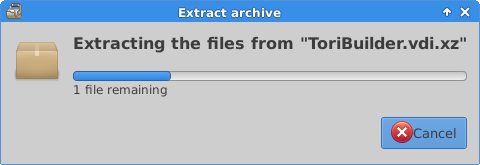
\includegraphics[width=0.7\linewidth]{extractVBimage}
\end{center}

Virtual box 
Click New

\begin{center}
\item 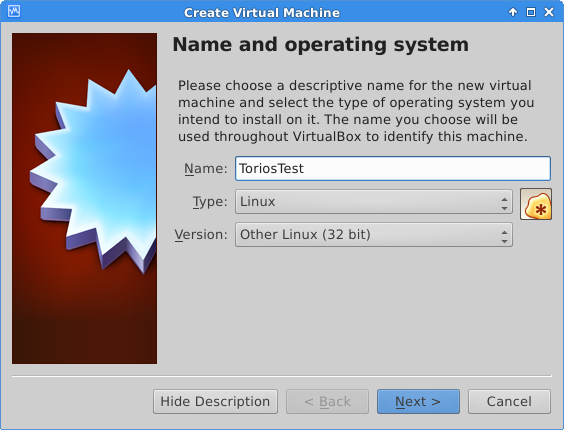
\includegraphics[width=0.7\linewidth]{ToriosTest01}
\end{center}

Use the following options
\begin{itemize}
\item Name : Torios
\item Type : Linux
\item Version : Ubuntu 32 bit
\end{itemize}

Click Next

\begin{center}
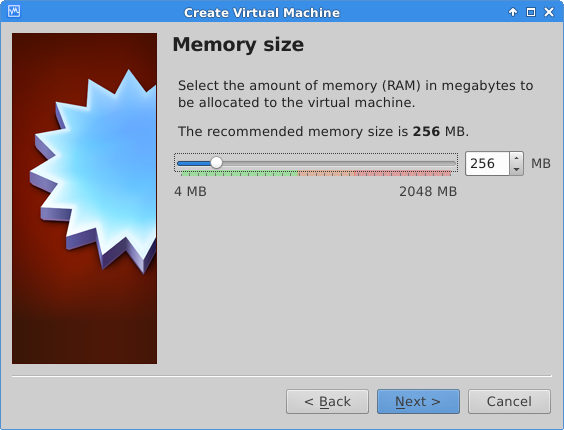
\includegraphics[width=0.7\linewidth]{ToriosTest02}
\end{center}

Should be Ok to leave the default memory as 256MB,so click next.

\begin{center}
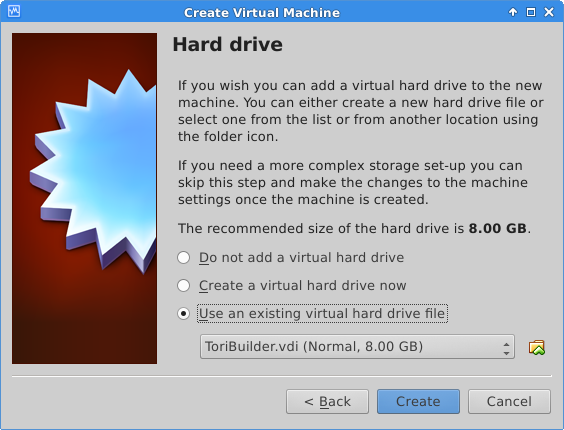
\includegraphics[width=0.7\linewidth]{ToriosTest03}
\end{center}

Upon opening virtual box you will see this screen:
\begin{center}
\includegraphics[width=0.7\linewidth]{virtualbox}
\end{center}

Click use existing and select the file you downloaded earlier, so in this case its \textbf{ToriBuilder.vdi}

Click done.

\begin{center}
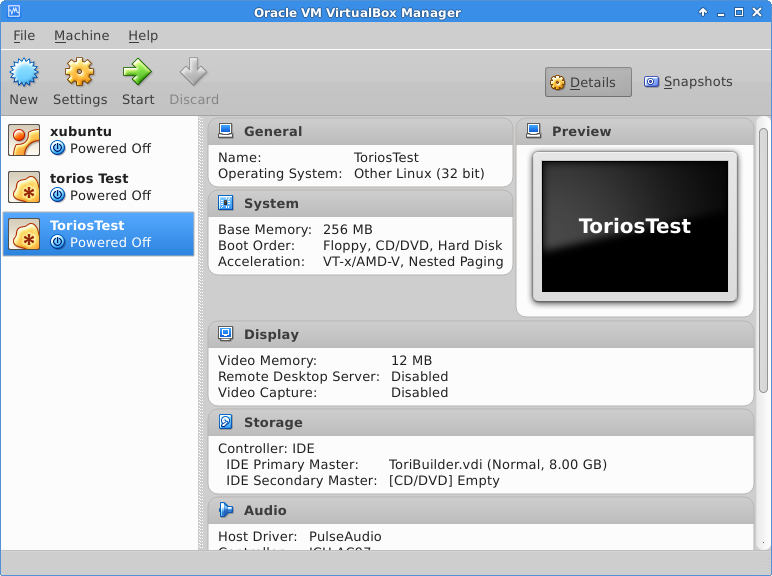
\includegraphics[width=0.7\linewidth]{ToriosTest-done}
\end{center}

Torios needs PAE support enabled to do this select the virtual box image you just created,  and click settings.

\begin{center}
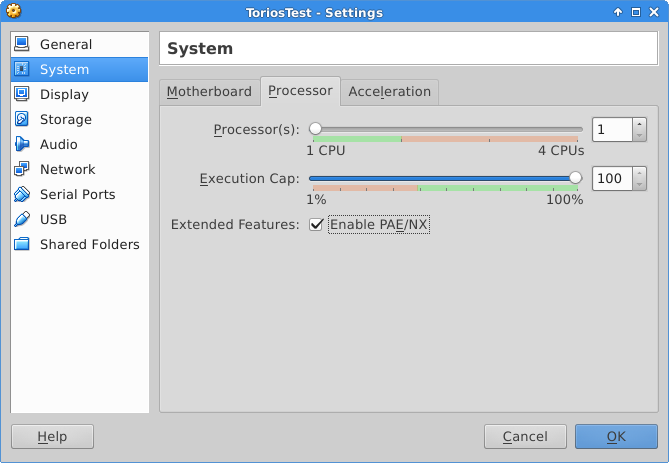
\includegraphics[width=0.7\linewidth]{ToriosEnablePAE}
\end{center}

Click system, then processor tab then check the box EnablePAE/NX then press OK.

You should then bereturned to the main virtual box window,  the image should still be selected so press start and you should boot in to the Torios Test Image. 

 note yours may look different as I have a few images,  also note in this screen shot i have a different vm set up.  We still need to open up the ToriOS image we downloaded. 

We will assume here you have thus already installed.


\chapter{Document License}
\index{Creative Commons}
\index{Document License}
\textbf{Attribution-ShareAlike 4.0 International (CC BY-SA 4.0)}

\begin{verbatim}
You are free to:

    Share ? copy and redistribute the material in any medium or format
    Adapt ? remix, transform, and build upon the material
    for any purpose, even commercially.

    The licensor cannot revoke these freedoms
     as long as you follow the license terms.


Under the following terms:

    Attribution ? You must give appropriate credit, provide a link to the license,
     and indicate if changes were made. 
     You may do so in any reasonable manner, 
     but not in any way that suggests the licensor endorses you or your use.

    ShareAlike ? If you remix, transform,
     or build upon the material, you must distribute your contributions under the same license as the original.

    No additional restrictions ? 
    You may not apply legal terms or technological 
    measures that legally restrict others from doing 
    anything the license permits.


\end{verbatim}

http://creativecommons.org/licenses/by-sa/4.0/

\chapter{Software License}
\index{Software License}
%\license[2.5]{by-nc-sa}
...
% images only
%\shortlicense[3.0]{by-nc-sa}
%\cc \ccby \ccsa

\chapter{URL References}
\index {URL References}
\label{URL REF}

\begin{center}\begin{tabular}{|l|l|}
\hline \textbf{Topic} & \textbf{URL} \\
\hline ToriOS Home Page & \htmladdnormallink{http://torios.org/}{http://torios.org/} \\

\hline ToriOS ISO & \htmladdnormallink{http://torios.org/ISO/ToriOS-alpha-rc2.iso}{http://torios.org/ISO/ToriOS-alpha-rc2.iso} \\

\hline Evince & \htmladdnormallink{https://wiki.gnome.org/Apps/Evince}{https://wiki.gnome.org/Apps/Evince} \\

\hline unetbootin & \htmladdnormallink{http://unetbootin.sourceforge.net/}{http://unetbootin.sourceforge.net/}\\

\hline mkusb & \htmladdnormallink{http://phillw.net/isos/linux-tools/mkusb/README.txt}{http://phillw.net/isos/linux-tools/mkusb/README.txt}\\

\hline Virtualboxx & \htmladdnormallink{https://www.virtualbox.org/}{https://www.virtualbox.org/}\\

\hline CC License & \htmladdnormallink{http://creativecommons.org/licenses/by-sa/4.0/}{http://creativecommons.org/licenses/by-sa/4.0/}\\


\hline \end{tabular}\end{center}




\chapter{PDF References}
\index{PDF References}
\label{PDF References}
\begin{center}\begin{tabular}{|l|l|}
\hline \textbf{PDF} & \textbf{Location} \\
\hline Quick start & \htmladdnormallink{mkUSB-quick-start-manual.pdf}{http://phillw.net/isos/linux-tools/mkusb/mkUSB-quick-start-manual.pdf} \\

\hline nox manual & \htmladdnormallink{mkUSB-quick-start-manual-nox.pdf}{http://phillw.net/isos/linux-tools/mkusb/mkUSB-quick-start-manual-nox.pdf} \\

\hline bas manual & \htmladdnormallink{mkUSB-quick-start-manual-bas.pdf}{http://phillw.net/isos/linux-tools/mkusb/mkUSB-quick-start-manual-bas.pdf} \\


\hline x & \htmladdnormallink{}{}\\

\hline x & \htmladdnormallink{}{}\\

\hline x & \htmladdnormallink{}{}\\

\hline x & \htmladdnormallink{}{}\\

\hline \end{tabular}\end{center}



\newpage






\printindex

\newpage


\end{document}